% !Rnw weave = knitr
\documentclass[a4paper, french, 11 pt]{article}\usepackage[]{graphicx}\usepackage[]{xcolor}
% maxwidth is the original width if it is less than linewidth
% otherwise use linewidth (to make sure the graphics do not exceed the margin)
\makeatletter
\def\maxwidth{ %
  \ifdim\Gin@nat@width>\linewidth
    \linewidth
  \else
    \Gin@nat@width
  \fi
}
\makeatother

\definecolor{fgcolor}{rgb}{0.345, 0.345, 0.345}
\newcommand{\hlnum}[1]{\textcolor[rgb]{0.686,0.059,0.569}{#1}}%
\newcommand{\hlstr}[1]{\textcolor[rgb]{0.192,0.494,0.8}{#1}}%
\newcommand{\hlcom}[1]{\textcolor[rgb]{0.678,0.584,0.686}{\textit{#1}}}%
\newcommand{\hlopt}[1]{\textcolor[rgb]{0,0,0}{#1}}%
\newcommand{\hlstd}[1]{\textcolor[rgb]{0.345,0.345,0.345}{#1}}%
\newcommand{\hlkwa}[1]{\textcolor[rgb]{0.161,0.373,0.58}{\textbf{#1}}}%
\newcommand{\hlkwb}[1]{\textcolor[rgb]{0.69,0.353,0.396}{#1}}%
\newcommand{\hlkwc}[1]{\textcolor[rgb]{0.333,0.667,0.333}{#1}}%
\newcommand{\hlkwd}[1]{\textcolor[rgb]{0.737,0.353,0.396}{\textbf{#1}}}%
\let\hlipl\hlkwb

\usepackage{framed}
\makeatletter
\newenvironment{kframe}{%
 \def\at@end@of@kframe{}%
 \ifinner\ifhmode%
  \def\at@end@of@kframe{\end{minipage}}%
  \begin{minipage}{\columnwidth}%
 \fi\fi%
 \def\FrameCommand##1{\hskip\@totalleftmargin \hskip-\fboxsep
 \colorbox{shadecolor}{##1}\hskip-\fboxsep
     % There is no \\@totalrightmargin, so:
     \hskip-\linewidth \hskip-\@totalleftmargin \hskip\columnwidth}%
 \MakeFramed {\advance\hsize-\width
   \@totalleftmargin\z@ \linewidth\hsize
   \@setminipage}}%
 {\par\unskip\endMakeFramed%
 \at@end@of@kframe}
\makeatother

\definecolor{shadecolor}{rgb}{.97, .97, .97}
\definecolor{messagecolor}{rgb}{0, 0, 0}
\definecolor{warningcolor}{rgb}{1, 0, 1}
\definecolor{errorcolor}{rgb}{1, 0, 0}
\newenvironment{knitrout}{}{} % an empty environment to be redefined in TeX

\usepackage{alltt}
\usepackage[T1]{fontenc}
\usepackage[utf8]{inputenc}
\usepackage{lmodern}
\usepackage{textcomp}
\usepackage[french]{babel}
\usepackage{geometry}
\geometry{top=1cm, bottom=1cm, left=1cm, right=1cm}
\usepackage{graphicx}
\usepackage{epstopdf}
\usepackage{booktabs}
\usepackage[skip=0.5\baselineskip]{caption}

\epstopdfDeclareGraphicsRule{.gif}{png}{.png}{convert gif:#1 png:\OutputFile}
\AppendGraphicsExtensions{.gif}
\usepackage{listings}
\usepackage{inconsolata}



\title{Titre provisoire}
\author{Louis Bourges, Jean-Baptiste Lagrange-Dupuis et Luc Letonturier}
\date{\today}
\IfFileExists{upquote.sty}{\usepackage{upquote}}{}
\begin{document}

\maketitle

Et ici on peut écrire ... et insérer des blocs de code qui s'éxécutent, avec le code et le résultat qui s'affichent

\begin{knitrout}
\definecolor{shadecolor}{rgb}{0.969, 0.969, 0.969}\color{fgcolor}\begin{kframe}
\begin{lstlisting}[basicstyle=\ttfamily,breaklines=true]
a <-  2+2\end{lstlisting}
\begin{lstlisting}[basicstyle=\ttfamily,breaklines=true]
a\end{lstlisting}
\begin{lstlisting}[basicstyle=\ttfamily,breaklines=true]
## [1] 4
\end{lstlisting}
\end{kframe}
\end{knitrout}

ou juste le résultat : 

\begin{knitrout}
\definecolor{shadecolor}{rgb}{0.969, 0.969, 0.969}\color{fgcolor}\begin{kframe}
\begin{lstlisting}[basicstyle=\ttfamily,breaklines=true]
## [1] 6
\end{lstlisting}
\end{kframe}
\end{knitrout}

ou totalement invisibles : 


Et ensuite on peut citer les résultats : à première vue $4 < 6$ mais je crois que c'est 8 qui est le plus grand.


Un petit graphique : 



\begin{figure}[h]
\center
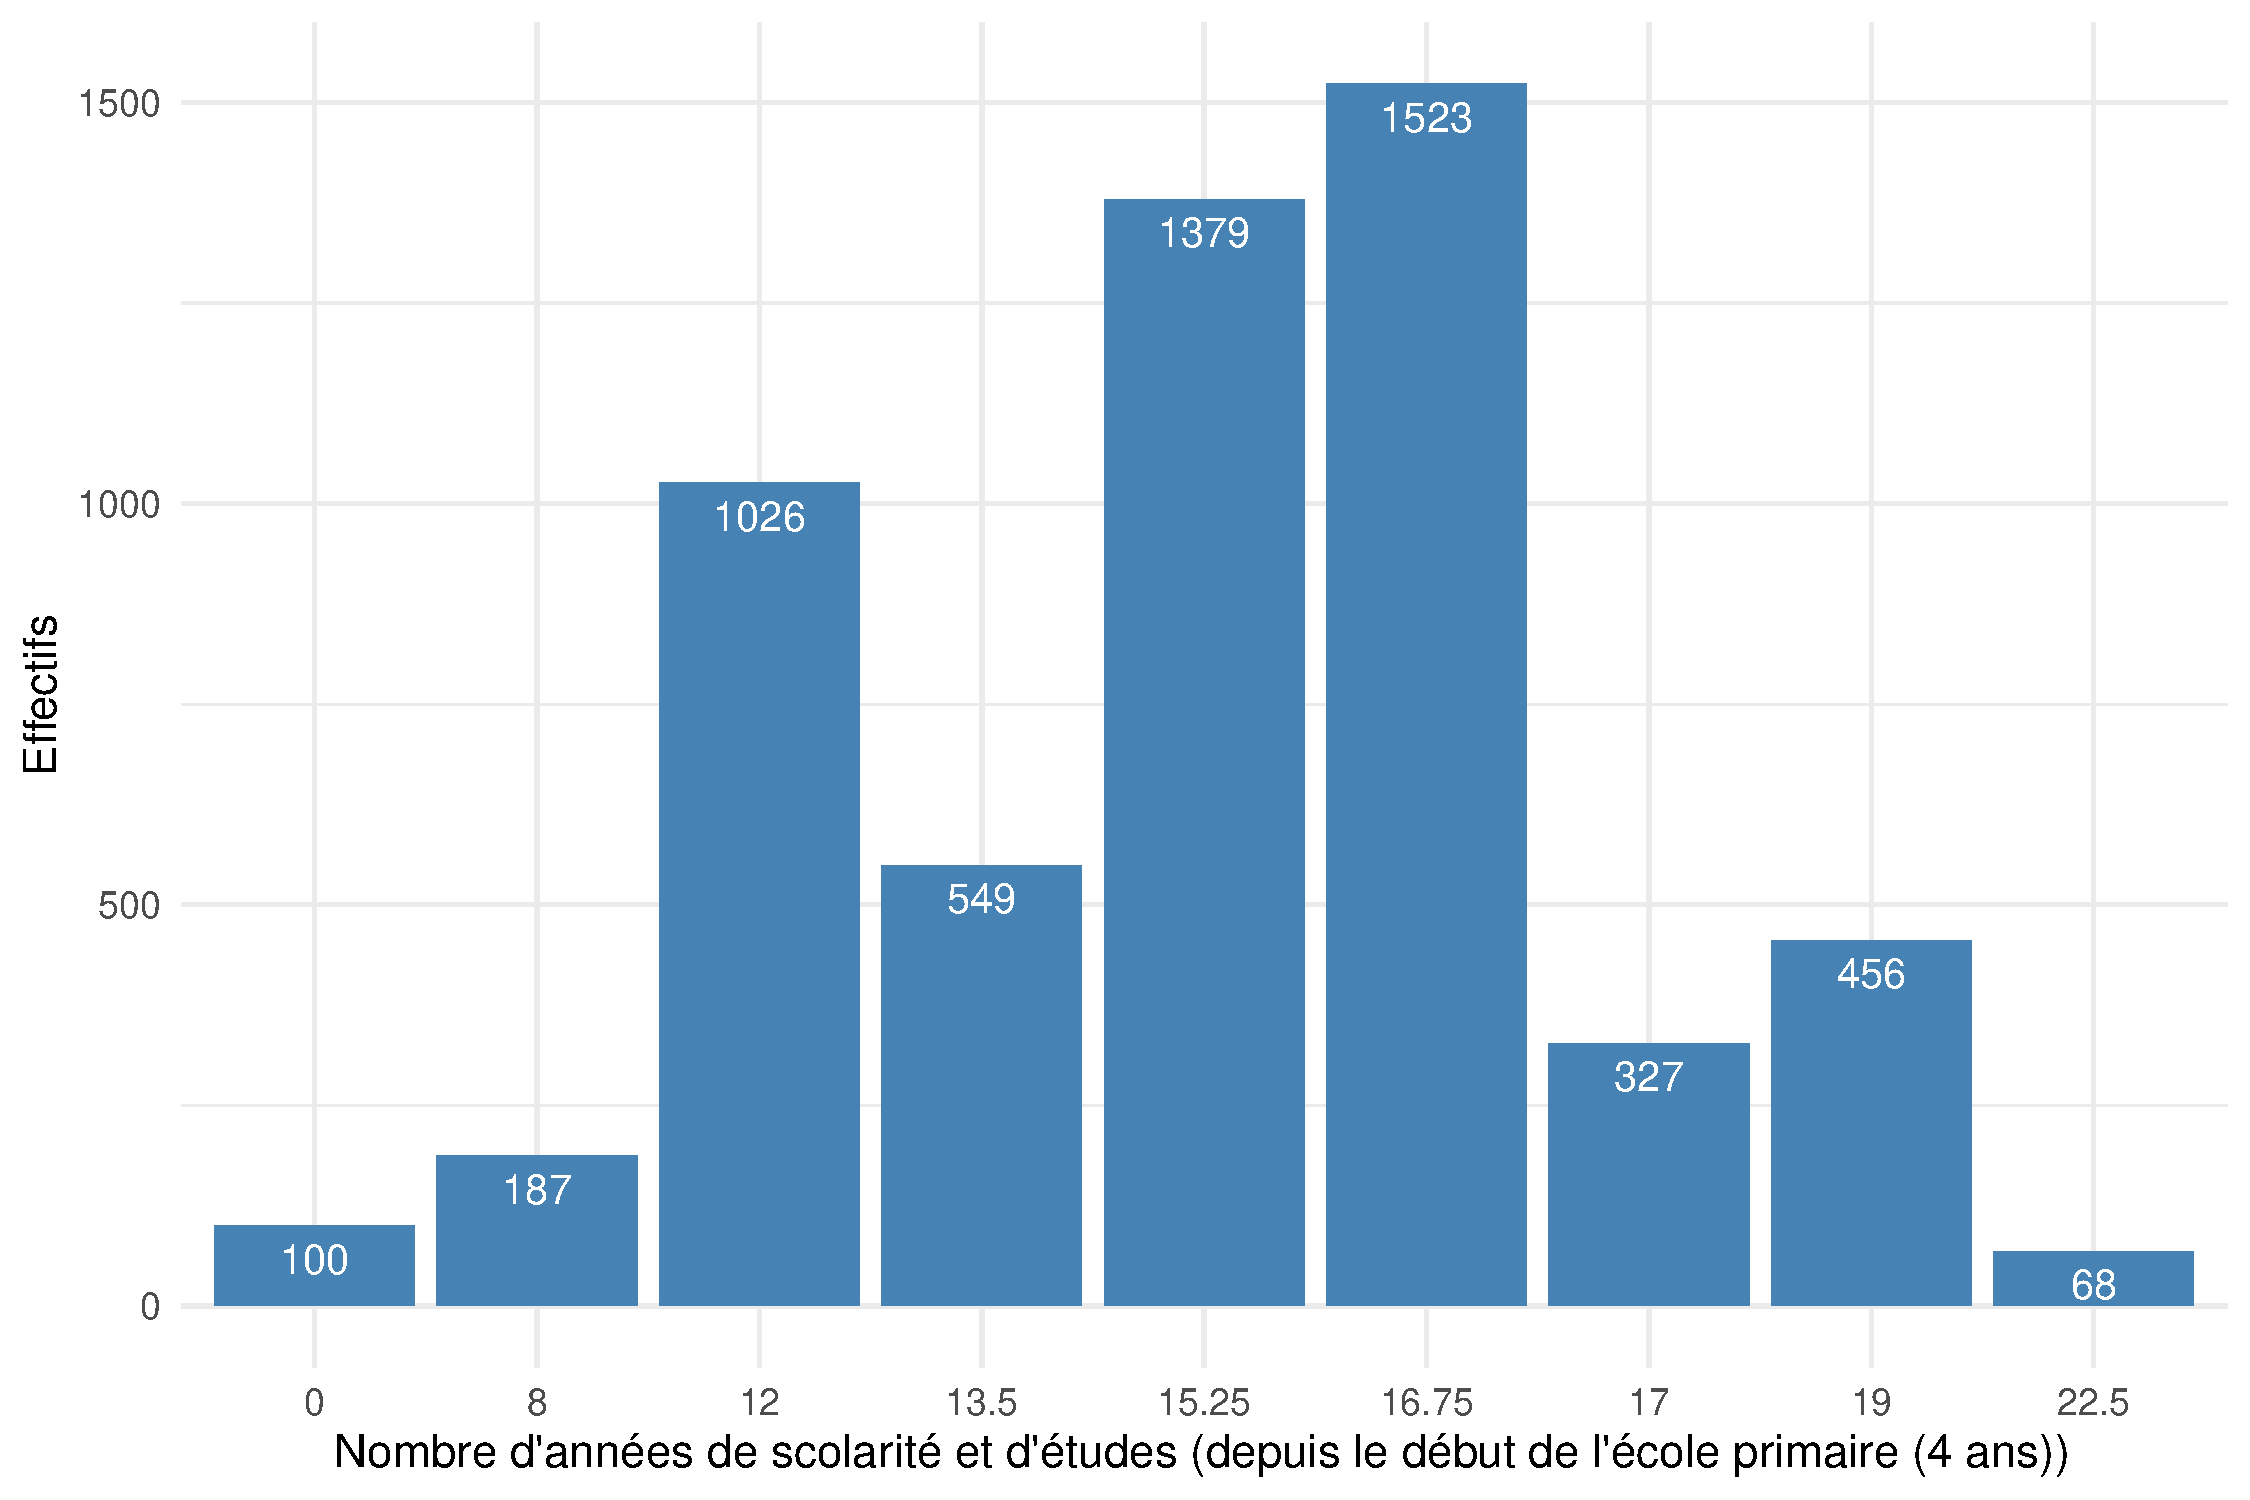
\includegraphics[width=0.7\linewidth]{figure/educ.pdf}
\caption{Niveau d'éducation (avec diplôme) des individus de l'échantillon}
\end{figure}

\begin{knitrout}
\definecolor{shadecolor}{rgb}{0.969, 0.969, 0.969}\color{fgcolor}\begin{kframe}
\begin{lstlisting}[basicstyle=\ttfamily,breaklines=true]
## [1] 5615
\end{lstlisting}
\begin{lstlisting}[basicstyle=\ttfamily,breaklines=true]
## [1] 0
\end{lstlisting}
\end{kframe}
\end{knitrout}


\begin{kframe}
\begin{lstlisting}[basicstyle=\ttfamily,breaklines=true]
% latex table generated in R 4.2.1 by xtable 1.8-4 package
% Sun May 14 12:07:52 2023
\begin{table}[ht]
\centering
\caption{Tableau des résidus} 
\label{tb:lm1}
\begin{tabular}{rrrrr}
  \toprule
 & Estimate & Std. Error & t value & Pr($>$$|$t$|$) \\ 
  \midrule
(Intercept) & 5.6786 & 0.1095 & 51.84 & 0.0000 \\ 
  data\$age & 0.0072 & 0.0010 & 7.11 & 0.0000 \\ 
  data\$genre & -0.3039 & 0.0225 & -13.53 & 0.0000 \\ 
  data\$heures & 0.0142 & 0.0008 & 17.03 & 0.0000 \\ 
  data\$experience & 0.0024 & 0.0011 & 2.15 & 0.0316 \\ 
  data\$nbenfants & -0.0097 & 0.0096 & -1.01 & 0.3112 \\ 
  data\$education & 0.1083 & 0.0059 & 18.44 & 0.0000 \\ 
   \bottomrule
\end{tabular}
\end{table}
\end{lstlisting}
\end{kframe}

Ici c'est l'annexe 

\begin{knitrout}
\definecolor{shadecolor}{rgb}{0.969, 0.969, 0.969}\color{fgcolor}\begin{kframe}
\begin{lstlisting}[basicstyle=\ttfamily,breaklines=true]
  options(width=60)\end{lstlisting}
\begin{lstlisting}[basicstyle=\ttfamily,breaklines=true]
\end{lstlisting}
\begin{lstlisting}[basicstyle=\ttfamily,breaklines=true]
  listing <- function(x, options) {
    paste("\\begin{lstlisting}[basicstyle=\\ttfamily,breaklines=true]\n",
      x, "\\end{lstlisting}\n", sep = "")
  }\end{lstlisting}
\begin{lstlisting}[basicstyle=\ttfamily,breaklines=true]
  knit_hooks$set(source=listing, output=listing)\end{lstlisting}
\begin{lstlisting}[basicstyle=\ttfamily,breaklines=true]
a <-  2+2\end{lstlisting}
\begin{lstlisting}[basicstyle=\ttfamily,breaklines=true]
a\end{lstlisting}
\begin{lstlisting}[basicstyle=\ttfamily,breaklines=true]
## [1] 4
\end{lstlisting}
\begin{lstlisting}[basicstyle=\ttfamily,breaklines=true]
b <-3+3\end{lstlisting}
\begin{lstlisting}[basicstyle=\ttfamily,breaklines=true]
b\end{lstlisting}
\begin{lstlisting}[basicstyle=\ttfamily,breaklines=true]
## [1] 6
\end{lstlisting}
\begin{lstlisting}[basicstyle=\ttfamily,breaklines=true]
c <- 4+4\end{lstlisting}
\begin{lstlisting}[basicstyle=\ttfamily,breaklines=true]
c\end{lstlisting}
\begin{lstlisting}[basicstyle=\ttfamily,breaklines=true]
## [1] 8
\end{lstlisting}
\begin{lstlisting}[basicstyle=\ttfamily,breaklines=true]
setwd("~/projet-econometrie-ensps")\end{lstlisting}
\begin{lstlisting}[basicstyle=\ttfamily,breaklines=true]
library(ggplot2)\end{lstlisting}
\begin{lstlisting}[basicstyle=\ttfamily,breaklines=true]
update_geom_defaults("text", list(size=30))\end{lstlisting}
\begin{lstlisting}[basicstyle=\ttfamily,breaklines=true]
library(xtable)\end{lstlisting}
\begin{lstlisting}[basicstyle=\ttfamily,breaklines=true]
                     \end{lstlisting}
\begin{lstlisting}[basicstyle=\ttfamily,breaklines=true]
                     \end{lstlisting}
\begin{lstlisting}[basicstyle=\ttfamily,breaklines=true]
###Importation des bases de données\end{lstlisting}
\begin{lstlisting}[basicstyle=\ttfamily,breaklines=true]
library(readr)\end{lstlisting}
\begin{lstlisting}[basicstyle=\ttfamily,breaklines=true]
library(ggplot2)\end{lstlisting}
\begin{lstlisting}[basicstyle=\ttfamily,breaklines=true]
school <- read_delim("data_LISS/work-and-school.csv", delim = ";", escape_double = FALSE, trim_ws = TRUE, show_col_types = FALSE)\end{lstlisting}


{\ttfamily\noindent\color{warningcolor}{\#\# Warning: One or more parsing issues, call `problems()` on your data\\\#\# frame for details, e.g.:\\\#\# \ \ dat <- vroom(...)\\\#\# \ \ problems(dat)}}\begin{lstlisting}[basicstyle=\ttfamily,breaklines=true]
background<-read_delim("data_LISS/avars_202207_EN_1.0p.csv", delim = ";", escape_double = FALSE, trim_ws = TRUE, show_col_types = FALSE)\end{lstlisting}
\begin{lstlisting}[basicstyle=\ttfamily,breaklines=true]
\end{lstlisting}
\begin{lstlisting}[basicstyle=\ttfamily,breaklines=true]
###Fusion des bases de données\end{lstlisting}
\begin{lstlisting}[basicstyle=\ttfamily,breaklines=true]
\end{lstlisting}
\begin{lstlisting}[basicstyle=\ttfamily,breaklines=true]
agregdata <- merge(background, school, by="nomem_encr" )\end{lstlisting}
\begin{lstlisting}[basicstyle=\ttfamily,breaklines=true]
\end{lstlisting}
\begin{lstlisting}[basicstyle=\ttfamily,breaklines=true]
###Gestion des NA\end{lstlisting}
\begin{lstlisting}[basicstyle=\ttfamily,breaklines=true]
\end{lstlisting}
\begin{lstlisting}[basicstyle=\ttfamily,breaklines=true]
#détection\end{lstlisting}
\begin{lstlisting}[basicstyle=\ttfamily,breaklines=true]
nrow(agregdata)\end{lstlisting}
\begin{lstlisting}[basicstyle=\ttfamily,breaklines=true]
## [1] 5723
\end{lstlisting}
\begin{lstlisting}[basicstyle=\ttfamily,breaklines=true]
agregdata <-  agregdata[!agregdata$oplzon==7,]#suppression de la catégorie "autre"\end{lstlisting}
\begin{lstlisting}[basicstyle=\ttfamily,breaklines=true]
\end{lstlisting}
\begin{lstlisting}[basicstyle=\ttfamily,breaklines=true]
nrow(agregdata)\end{lstlisting}
\begin{lstlisting}[basicstyle=\ttfamily,breaklines=true]
## [1] 5670
\end{lstlisting}
\begin{lstlisting}[basicstyle=\ttfamily,breaklines=true]
sum(is.na(agregdata$oplzon))\end{lstlisting}
\begin{lstlisting}[basicstyle=\ttfamily,breaklines=true]
## [1] 0
\end{lstlisting}
\begin{lstlisting}[basicstyle=\ttfamily,breaklines=true]
sum(agregdata$oplzon==8)\end{lstlisting}
\begin{lstlisting}[basicstyle=\ttfamily,breaklines=true]
## [1] 0
\end{lstlisting}
\begin{lstlisting}[basicstyle=\ttfamily,breaklines=true]
#aucun na à priori\end{lstlisting}
\begin{lstlisting}[basicstyle=\ttfamily,breaklines=true]
\end{lstlisting}
\begin{lstlisting}[basicstyle=\ttfamily,breaklines=true]
###Pré-traitement des données et réécriture des variables (a.e = années d'études)\end{lstlisting}
\begin{lstlisting}[basicstyle=\ttfamily,breaklines=true]
\end{lstlisting}
\begin{lstlisting}[basicstyle=\ttfamily,breaklines=true]
#On s'appuie d'abord sur la variable oplzon (niveau d'études "with diploma")\end{lstlisting}
\begin{lstlisting}[basicstyle=\ttfamily,breaklines=true]
agregdata$educ <- agregdata$oplmet*100\end{lstlisting}
\begin{lstlisting}[basicstyle=\ttfamily,breaklines=true]
agregdata$educ <- ifelse(agregdata$educ==800|agregdata$educ==900, 0,
                         #pas d'études du tout : "Not yet completed any education" or "Not (yet) started any education"
                         ifelse(agregdata$educ==100, 8,
                                #primary de 4 à 12 ans => 8 ans d'études : primary school
                                ifelse(agregdata$educ==200, 12,
                                       #1st option : VMBO (4 ans, de 12 à 16) => 8+4=12 a.e. : "vmbo (intermediate secondary education, US: junior high school)"
                                       ifelse(agregdata$educ==300, 13.5,
                                              #2nd option : HAVO (5 ans, de 12 à 17) or VWO (6 ans, de 12 à 18) => 8+5,5 = 13.5 a.e. : "havo/vwo (higher secondary education/preparatory university education, US: senior high school)"
                                              ifelse(agregdata$educ==400, 15.25,
                                                     #1st option : MBO (entre 1 et 4 ans, après VMBO, HAVO ou VWO) => 12.75 + 2.5 = 15.25 a.e. : "mbo (intermediate vocational education, US: junior college)"
                                                     ifelse(agregdata$educ==500, 16.75,
                                                            #2nd option : HBO (4 ans, après VMBO, HAVO ou VWO) => 12.75+4=16.75 a.e. : "hbo (higher vocational education, US: college)"
                                                            ifelse(agregdata$educ==600, 17, -9)))))))\end{lstlisting}
\begin{lstlisting}[basicstyle=\ttfamily,breaklines=true]
#3rd option : WO (3 ans, après 1ere année HBO (13.75 a.e.) ou après VWO (14 a.e.), licence) => 14+3=17 a.e. : "wo (university)"\end{lstlisting}
\begin{lstlisting}[basicstyle=\ttfamily,breaklines=true]
nrow(agregdata)\end{lstlisting}
\begin{lstlisting}[basicstyle=\ttfamily,breaklines=true]
## [1] 5670
\end{lstlisting}
\begin{lstlisting}[basicstyle=\ttfamily,breaklines=true]
sum(agregdata$educ==-9)\end{lstlisting}
\begin{lstlisting}[basicstyle=\ttfamily,breaklines=true]
## [1] 55
\end{lstlisting}
\begin{lstlisting}[basicstyle=\ttfamily,breaklines=true]
agregdata <-  agregdata[!agregdata$educ==-9,]\end{lstlisting}
\begin{lstlisting}[basicstyle=\ttfamily,breaklines=true]
nrow(agregdata)\end{lstlisting}
\begin{lstlisting}[basicstyle=\ttfamily,breaklines=true]
## [1] 5615
\end{lstlisting}
\begin{lstlisting}[basicstyle=\ttfamily,breaklines=true]
#Puis, pour distinguer entre licence, master et doctorat, on s'appuie sur la variable cw22o005 :\end{lstlisting}
\begin{lstlisting}[basicstyle=\ttfamily,breaklines=true]
sum(agregdata$cw22o005==27) #nombre de titulaires d'un PhD\end{lstlisting}
\begin{lstlisting}[basicstyle=\ttfamily,breaklines=true]
## [1] 68
\end{lstlisting}
\begin{lstlisting}[basicstyle=\ttfamily,breaklines=true]
sum(agregdata$cw22o005==26) #nombre de titulaires d'un master (au maximum)\end{lstlisting}
\begin{lstlisting}[basicstyle=\ttfamily,breaklines=true]
## [1] 456
\end{lstlisting}
\begin{lstlisting}[basicstyle=\ttfamily,breaklines=true]
sum(agregdata$cw22o005==25) #nombre de titulaires d'une licence (au maximum)\end{lstlisting}
\begin{lstlisting}[basicstyle=\ttfamily,breaklines=true]
## [1] 117
\end{lstlisting}
\begin{lstlisting}[basicstyle=\ttfamily,breaklines=true]
sum(agregdata$cw22o005==27)+sum(agregdata$cw22o005==26)+sum(agregdata$cw22o005==25) #nombre de diplômés du supérieur (au moins licence), selon cw22o005\end{lstlisting}
\begin{lstlisting}[basicstyle=\ttfamily,breaklines=true]
## [1] 641
\end{lstlisting}
\begin{lstlisting}[basicstyle=\ttfamily,breaklines=true]
sum(agregdata$educ==18)\end{lstlisting}
\begin{lstlisting}[basicstyle=\ttfamily,breaklines=true]
## [1] 0
\end{lstlisting}
\begin{lstlisting}[basicstyle=\ttfamily,breaklines=true]
sum((agregdata$cw22o005==27|agregdata$cw22o005==26|agregdata$cw22o005==25)&agregdata$educ!=17)#nombre d'observations "bizarres"\end{lstlisting}
\begin{lstlisting}[basicstyle=\ttfamily,breaklines=true]
## [1] 62
\end{lstlisting}
\begin{lstlisting}[basicstyle=\ttfamily,breaklines=true]
#On considère que les réponses à la question cw22o005 sont plus fiables car plus précises.\end{lstlisting}
\begin{lstlisting}[basicstyle=\ttfamily,breaklines=true]
\end{lstlisting}
\begin{lstlisting}[basicstyle=\ttfamily,breaklines=true]
\end{lstlisting}
\begin{lstlisting}[basicstyle=\ttfamily,breaklines=true]
\end{lstlisting}
\begin{lstlisting}[basicstyle=\ttfamily,breaklines=true]
agregdata$educ2 <- ifelse(agregdata$cw22o005==25, 17,
                         #niveau licence => 18 ans d'études
                         ifelse(agregdata$cw22o005==26, 19,
                                #niveau master, le master dure 1, 2 ou 3 ans => 17 + 2 = 19 a.e.
                                ifelse(agregdata$cw22o005==27, 22.5, agregdata$educ))) #après le master, un doctorat dure 3 à 4 ans => 19 + 3.5 = 22.5 a.e.\end{lstlisting}
\begin{lstlisting}[basicstyle=\ttfamily,breaklines=true]
\end{lstlisting}
\begin{lstlisting}[basicstyle=\ttfamily,breaklines=true]
\end{lstlisting}
\begin{lstlisting}[basicstyle=\ttfamily,breaklines=true]
g <- ggplot(agregdata, aes(x=factor(agregdata$educ2)), id=id, transition=TRUE)+
  geom_bar(fill="steelblue")+
  labs(x="Nombre d'années de scolarité et d'études (depuis le début de l'école primaire (4 ans))", y = "Effectifs")+
  geom_text(stat='count', aes(label=after_stat(count)), vjust=1.6, color="white", size=7)+
  theme_minimal(base_size = 22)\end{lstlisting}
\begin{lstlisting}[basicstyle=\ttfamily,breaklines=true]
ggsave(g, filename = "figure/educ.pdf", width=15, height=10)\end{lstlisting}


{\ttfamily\noindent\bfseries\color{errorcolor}{\#\# Error in grDevices::pdf(file = filename, ..., version = version): cannot open file 'figure/educ.pdf'}}\begin{lstlisting}[basicstyle=\ttfamily,breaklines=true]
###Création d'une table avec les données pertinentes\end{lstlisting}
\begin{lstlisting}[basicstyle=\ttfamily,breaklines=true]
\end{lstlisting}
\begin{lstlisting}[basicstyle=\ttfamily,breaklines=true]
data<-data.frame(agregdata$nomem_encr,agregdata$leeftijd,agregdata$geslacht,agregdata$brutoink,agregdata$cw22o127,agregdata$cw22o134, agregdata$educ, agregdata$aantalki)\end{lstlisting}
\begin{lstlisting}[basicstyle=\ttfamily,breaklines=true]
names(data)<-c("identite", "age", "genre", "revenu", "heures", "experience","education", "nbenfants")\end{lstlisting}
\begin{lstlisting}[basicstyle=\ttfamily,breaklines=true]
\end{lstlisting}
\begin{lstlisting}[basicstyle=\ttfamily,breaklines=true]
nrow(data)\end{lstlisting}
\begin{lstlisting}[basicstyle=\ttfamily,breaklines=true]
## [1] 5615
\end{lstlisting}
\begin{lstlisting}[basicstyle=\ttfamily,breaklines=true]
sum(is.na(data$nbenfants))\end{lstlisting}
\begin{lstlisting}[basicstyle=\ttfamily,breaklines=true]
## [1] 0
\end{lstlisting}
\begin{lstlisting}[basicstyle=\ttfamily,breaklines=true]
data <-  data[!data$revenu<=0,]\end{lstlisting}
\begin{lstlisting}[basicstyle=\ttfamily,breaklines=true]
data <- data[!is.na(data$heures),]\end{lstlisting}
\begin{lstlisting}[basicstyle=\ttfamily,breaklines=true]
data <- data[!is.na(data$experience),]\end{lstlisting}
\begin{lstlisting}[basicstyle=\ttfamily,breaklines=true]
data <- data[!is.na(data$education),]\end{lstlisting}
\begin{lstlisting}[basicstyle=\ttfamily,breaklines=true]
data <-  data[!data$experience==999,]\end{lstlisting}
\begin{lstlisting}[basicstyle=\ttfamily,breaklines=true]
data <-  data[!data$education==-9,]\end{lstlisting}
\begin{lstlisting}[basicstyle=\ttfamily,breaklines=true]
data <-  data[!data$heures==999,]\end{lstlisting}
\begin{lstlisting}[basicstyle=\ttfamily,breaklines=true]
data <-  data[!data$genre==3,]\end{lstlisting}
\begin{lstlisting}[basicstyle=\ttfamily,breaklines=true]
\end{lstlisting}
\begin{lstlisting}[basicstyle=\ttfamily,breaklines=true]
###Réecriture des variables : \end{lstlisting}
\begin{lstlisting}[basicstyle=\ttfamily,breaklines=true]
\end{lstlisting}
\begin{lstlisting}[basicstyle=\ttfamily,breaklines=true]
data$genre <- ifelse(data$genre==1, 0, 1)\end{lstlisting}
\begin{lstlisting}[basicstyle=\ttfamily,breaklines=true]
data$log_revenu <- log(data$revenu)\end{lstlisting}
\begin{lstlisting}[basicstyle=\ttfamily,breaklines=true]
\end{lstlisting}
\begin{lstlisting}[basicstyle=\ttfamily,breaklines=true]
\end{lstlisting}
\begin{lstlisting}[basicstyle=\ttfamily,breaklines=true]
data$experience <- 2022 - data$experience\end{lstlisting}
\begin{lstlisting}[basicstyle=\ttfamily,breaklines=true]
\end{lstlisting}
\begin{lstlisting}[basicstyle=\ttfamily,breaklines=true]
\end{lstlisting}
\begin{lstlisting}[basicstyle=\ttfamily,breaklines=true]
lm1 <- lm(data$log_revenu ~ data$age + data$genre + data$heures + data$experience + data$nbenfants + data$education)\end{lstlisting}
\begin{lstlisting}[basicstyle=\ttfamily,breaklines=true]
\end{lstlisting}
\begin{lstlisting}[basicstyle=\ttfamily,breaklines=true]
print(xtable(summary(lm1), caption="Tableau des résidus", label="tb:lm1"), booktabs=TRUE, caption.placement="top")\end{lstlisting}
\begin{lstlisting}[basicstyle=\ttfamily,breaklines=true]
## % latex table generated in R 4.2.1 by xtable 1.8-4 package
## % Sun May 14 12:07:53 2023
## \begin{table}[ht]
## \centering
## \caption{Tableau des résidus} 
## \label{tb:lm1}
## \begin{tabular}{rrrrr}
##   \toprule
##  & Estimate & Std. Error & t value & Pr($>$$|$t$|$) \\ 
##   \midrule
## (Intercept) & 5.6786 & 0.1095 & 51.84 & 0.0000 \\ 
##   data\$age & 0.0072 & 0.0010 & 7.11 & 0.0000 \\ 
##   data\$genre & -0.3039 & 0.0225 & -13.53 & 0.0000 \\ 
##   data\$heures & 0.0142 & 0.0008 & 17.03 & 0.0000 \\ 
##   data\$experience & 0.0024 & 0.0011 & 2.15 & 0.0316 \\ 
##   data\$nbenfants & -0.0097 & 0.0096 & -1.01 & 0.3112 \\ 
##   data\$education & 0.1083 & 0.0059 & 18.44 & 0.0000 \\ 
##    \bottomrule
## \end{tabular}
## \end{table}
\end{lstlisting}
\end{kframe}
\end{knitrout}

\end{document}
